\documentclass[12pt,letterpaper]{article}
\usepackage[margin=1in]{geometry}
\usepackage{chngpage}
\usepackage[english]{babel}
\usepackage[utf8x]{inputenc}
\usepackage{amsmath}
\usepackage{amssymb} 
% \usepackage[retainorgcmds]{IEEEtrantools}
\usepackage{graphicx}
\usepackage{tabularx}
\usepackage{kpfonts}    % for nice fonts
\usepackage{microtype} 
\usepackage{booktabs}   % for nice tables
\usepackage{bm}         % for bold math
\usepackage{listings}   % for inserting code
\usepackage{verbatim}   % useful for program listings
\usepackage{color}  
\usepackage[colorlinks=true]{hyperref}
% use for hypertext
\hypersetup{
	colorlinks=false,       % false: boxed links; true: colored links
	linkcolor=green,        % color of internal links
	citecolor=blue,        % color of links to bibliography
	filecolor=magenta,     % color of file links
	urlcolor=blue         
}
\usepackage[colorinlistoftodos]{todonotes}
\usepackage{natbib}
\usepackage{float}
\usepackage{adjustbox}
\usepackage[capitalise]{cleveref}
\usepackage{xcolor}

\usepackage{longtable,threeparttablex}
\usepackage{subcaption}



%++++++++++++++++++++++++++++++++++++++++


\begin{document}

\begin{center}
\large IEMS-469 Dynamic Programming  HW3

\bigskip
Weijia Zhao \footnote{Weijia.Zhao@kellogg.northwestern.edu}\\
Kellogg Finance

\bigskip
This version: \today
\end{center}

\newpage
Outline: Due to the difficulties to access Deepdish computing resources (too crowded) and the fact that I cannot move files using either Cyberduck/FileZilla (says I am not authorized to do so), I use Northwestern Quest for the training of question (b) Pacman-v0 in this homework assignment. (I have an existing type I account and the GPU used for this homework is A100). (You can also find a copy on Google Colab \href{https://colab.research.google.com/drive/1990i7SjLFgfk_CTRvJBCWppqFl8RlDNg?usp=sharing}{HERE}). Question (a) is fairly easy and the computation is extremely fast even just using CPU.\\

I use a moving average with a constant decay rate to calculate the average reward versus training epochs rather than only consider the most recent 10 epochs or so as
\begin{itemize}
\item (1) Moving average technically takes into account all historical episodes and is less random than the average of 10 most recent epochs (eg: when you just get 10 consecutive good results by luck)
\item (2) Moving average can be easily implemented iteratively along with the training process with lower computational effort: $MA_t=(1-\alpha)MA_{t-1}+\alpha R_t$
\end{itemize}

The network structure used for each problem is:
\begin{itemize}
\item (Cartpole): Fully connected$\rightarrow$Relu$\rightarrow$Fully connected
\item (Pacman): Following what you showed in TA session, I first stack four steps of graphs (i.e. four input channels) together\footnote{Technically this is not necessary since we are able to identify the direction of the Pacman just based on one single screenshot. However, I feel that the difference in direction is so small in a graph and the neural network may not be able to successfully pick up this feature so stacking seems to be } as each individual block. Then Convolution with kernel 5 stride 2 output channel 16$\rightarrow$Batch Normalization$\rightarrow$Relu$\rightarrow$ Convolution with kernel 5 stride 2 output channel 32$\rightarrow$Batch Normalization$\rightarrow$Relu$\rightarrow$Convolution with kernel 5 stride 2 output channel 32$\rightarrow$Batch Normalization$\rightarrow$Relu$\rightarrow$ Fully connected$\rightarrow$Relu$\rightarrow$Fully Connected (output dim=1
\end{itemize}

\section{Cartpole}
As mentioned, this model is trained with CPU due to its simplicity. I did not try to optimize the hyperparameter in this question as it converges within 5 (mostly related to the decaying speed of $\epsilon$) or several minutes even in the worst case scenario. (The smooth coefficient here is $\alpha=0.1$)\\

The plot of individual epoch reward is given in the following graph: as expected, deep q network is also quite volatile. My initial value for the moving average smoother is 0 (so we should ignore the first maybe 50 episodes as the increase in q-value or reward there is just due to the fact that the starting value of the moving average is too small). Also I would like to mention that even after reaching the best, there is still the possibility that reward goes down or fluctuate following some particular episodes and then recover later (i.e. the convergence is stochastic rather than deterministic). This pattern is reflected in the graph for testing, we can see that in many cases we get 200, but we also sometimes get lower total rewards, such as 150, 180 etc, and the average score is more like 175-180. Recall that the average reward following a random policy is about 20, so indeed our algorithm learns how to play the game.




 \begin{figure}[H]
 	\centering
 	\caption{Cartpole game}
 	\begin{subfigure}[h]{0.9\textwidth}
 		\centering
 		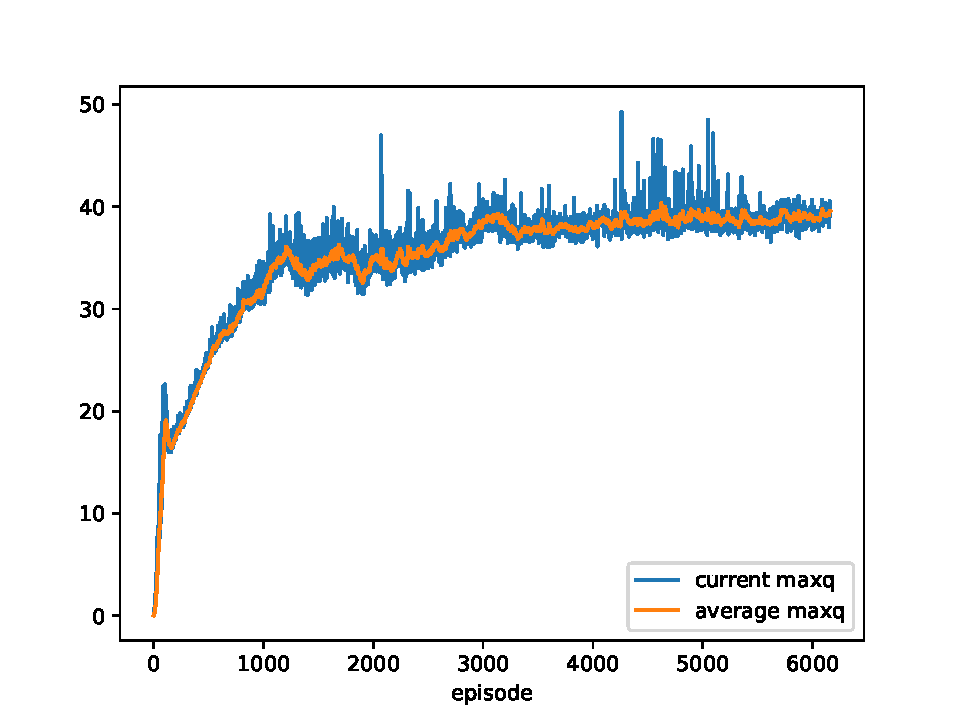
\includegraphics[width=\textwidth]{/Users/lesliezhao/Dropbox/nu_course/2021_fall/DP/IEMS469_HW_LWZ/hw3/1_cartpole_qvalue.pdf}
 		\caption{Training: qvalue}
 	\end{subfigure}
  	\begin{subfigure}[h]{0.9\textwidth}
 	\centering
 	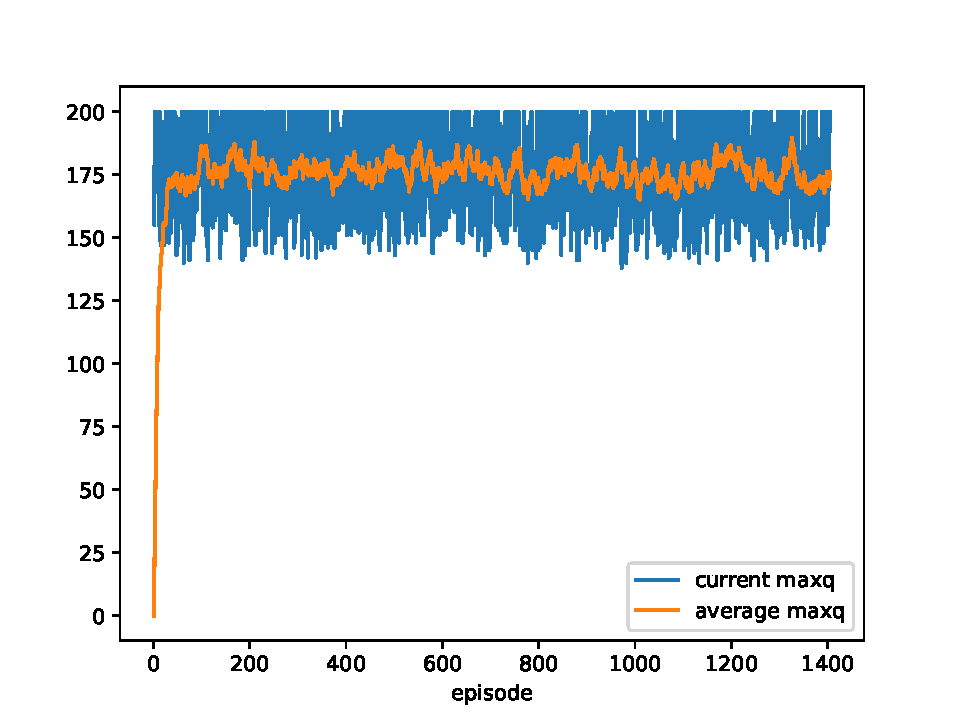
\includegraphics[width=\textwidth]{/Users/lesliezhao/Dropbox/nu_course/2021_fall/DP/IEMS469_HW_LWZ/hw3/1_cartpole_reward.pdf}
 	\caption{Testing: reward}
 \end{subfigure}
 \end{figure}


\section{Pacman}
As mentioned, I train the model with Northwestern Quest due to the inaccessibility of Deepdish (You can also find a copy on Google Colab \href{https://colab.research.google.com/drive/1990i7SjLFgfk_CTRvJBCWppqFl8RlDNg?usp=sharing}{HERE}). I use a relatively small learning rate 1e-5 after some trials. (Again the smooth factor here is $\alpha=0.1$, unfortunately, this seems to be too large given that the volatility of Q value is extremely high, so even the moving average is still very volatile....I should try a smaller $\alpha$)\\

For exploration v.s. exploitation, I start the epsilon from 1 (i.e. full exploration) and use a linear decay until 0.05, while the decay rate is given by the total number of steps divided by 10,000,000 (on average, one single episode contains about 700 steps to finish, so this corresponds to about 14500 episodes). After reaching 0.05, the exploration rate stays constant. \\

Unfortunately, the performance of the algorithm seems to decline a bit at the end of the training. I was expecting the reward to increase whenever the maxq increases, but this is not really the case. Some possible reasons may just be that there is too much randomness in the game and the computer chooses different strategies all the time (i.e. whether the enemy will chase our agent), so even if we find a particular state-action pair to be very good in this episode, it may not be the case the next time. Since I make a copy of the neural network parameters every 100 episodes, I instead choose the best model available (episode around 16000). \\

I am not quite sure about the capability of DQN in playing this Pacman game, but I was a bit disappointed in the sense that even the best model (with a relatively complex structure) here 
can only get an average reward of 680. On the other hand, I do see reward can be over 2000 in some episodes, so seems to be it is still far from optimal (I am not very clear but seems to me the maximal reward possible in this game can be over 100000? If that is the case, then there must be a huge space for improvement...But I did not have enough time waiting for the model to train another maybe 200000 episodes, neither did I try enough different random seed or tune the parameters, maybe those are the reasons why my model does not give me very outstanding performance) 

 \begin{figure}[H]
	\centering
	\caption{Pacman game}
	\begin{subfigure}[h]{0.9\textwidth}
		\centering
		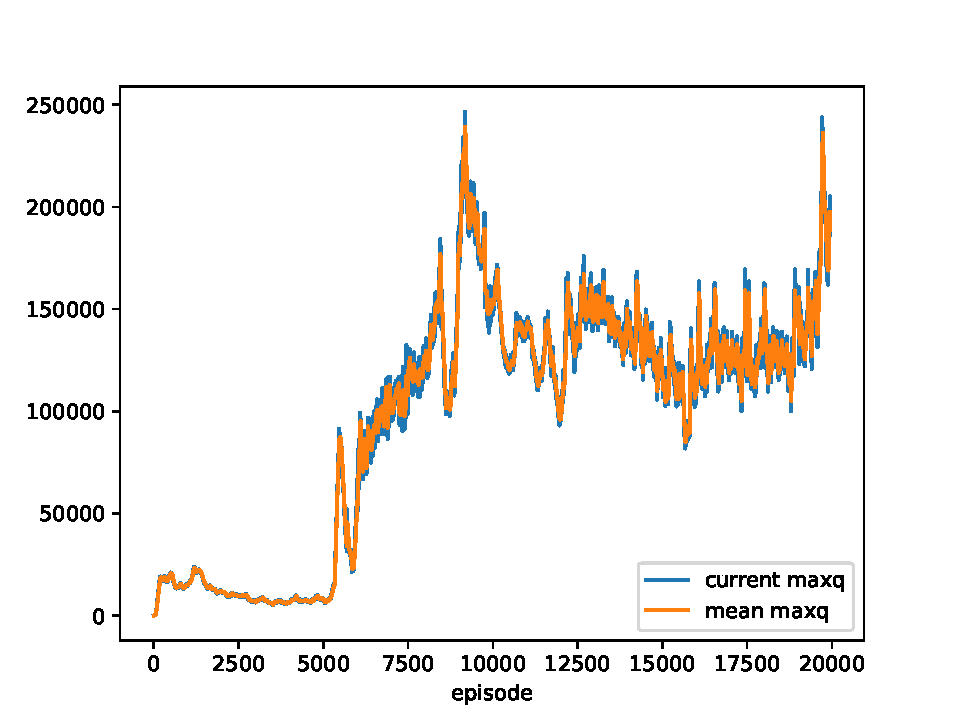
\includegraphics[width=\textwidth]{/Users/lesliezhao/Dropbox/nu_course/2021_fall/DP/IEMS469_HW_LWZ/hw3/2_pacman_qvalue.pdf}
		\caption{Training: qvalue}
	\end{subfigure}
	\begin{subfigure}[h]{0.9\textwidth}
	\centering
	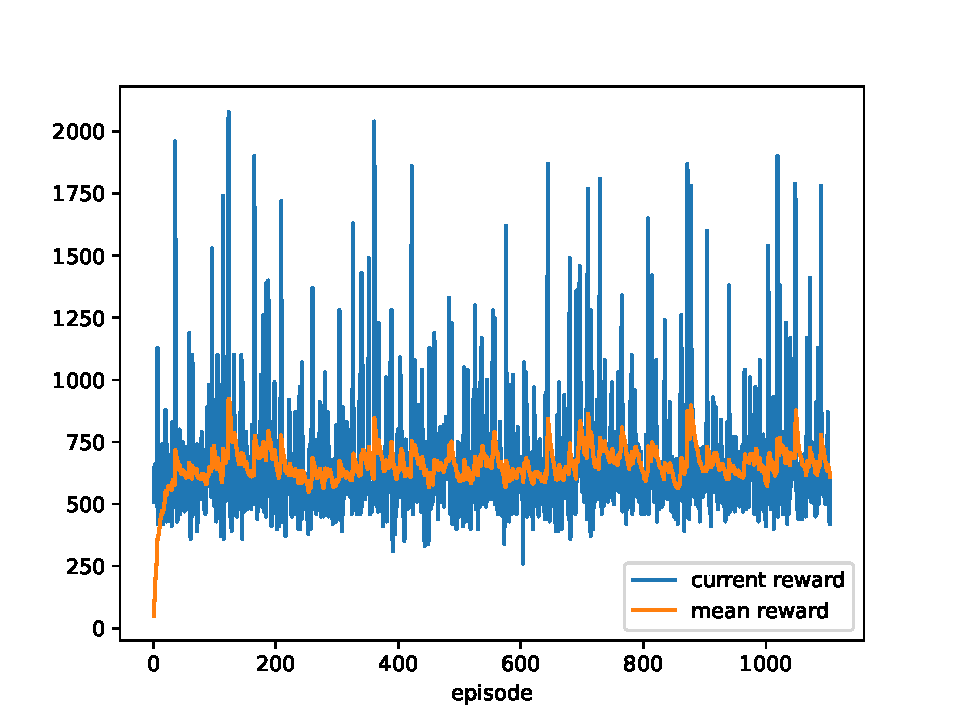
\includegraphics[width=\textwidth]{/Users/lesliezhao/Dropbox/nu_course/2021_fall/DP/IEMS469_HW_LWZ/hw3/2_pacman_reward.pdf}
	\caption{Training: reward}
\end{subfigure}
\end{figure}



\end{document}
